\documentclass[a4paper,12pt]{article}
\addtolength{\oddsidemargin}{-1.cm}
\addtolength{\textwidth}{2cm}
\addtolength{\topmargin}{-3cm}
\addtolength{\textheight}{3.5cm}
\makeindex


\usepackage[pdftex]{graphicx}
\usepackage{makeidx}
\usepackage{float}
\usepackage{hyperref}
\hypersetup{
	colorlinks=true,
	linkcolor=blue,
	filecolor=magenta,      
	urlcolor=cyan,
}



% define the title
\author{CodeBlox}
\title{Tender}
\begin{document}
	\setlength{\parskip}{6pt}
	
	% generates the title
	\begin{titlepage}
		\begin{center}
			
\includegraphics[width=1\textwidth]{./Pictures/up_logo.png}\\[1.5cm] 
			\textsc{\LARGE Department of Computer Science} \\ [.5cm]
			\textsc{\Large User Manual} \\ [.5cm]
			\line(1,0){450}\\[.5cm]
			\huge{\bfseries Client: Gavin Potgieter}\\
			\line(1,0){450}\\[.5cm]
			\textsc{\LARGE Team: CodeBlox}\\ [0.5cm]
			
			
			\textsc{\large Lethabo Mogase (Bsc: Computer Science)}\\
			\textsc{\large Lorenzo Spazzoli (Bsc: Computer Science)}\\
			\textsc{\large Bilal Muhammad (BIS: Multimedia)}\\
			\textsc{\large Dirk de Klerk (BIS: Multimedia)}\\ [3.9cm]
			
			\large\today
		\end{center}
	\end{titlepage}
	
	\tableofcontents
	\thispagestyle{empty}
	\footnotesize
	\normalsize
	
	
	
	
	\newpage
	\section{System Overview}
	The main objective of this system is to allow a delivery person into a demarcated area of your house when you are not there. You should be able to give access remotely and monitor the delivery person while you are not in the area. 
	The project has been named "DropOff" and has been persued by team CodeBlox.
	
	This document will demonstrate how the user would use the system.
	
	\section{System Configuration}
		
		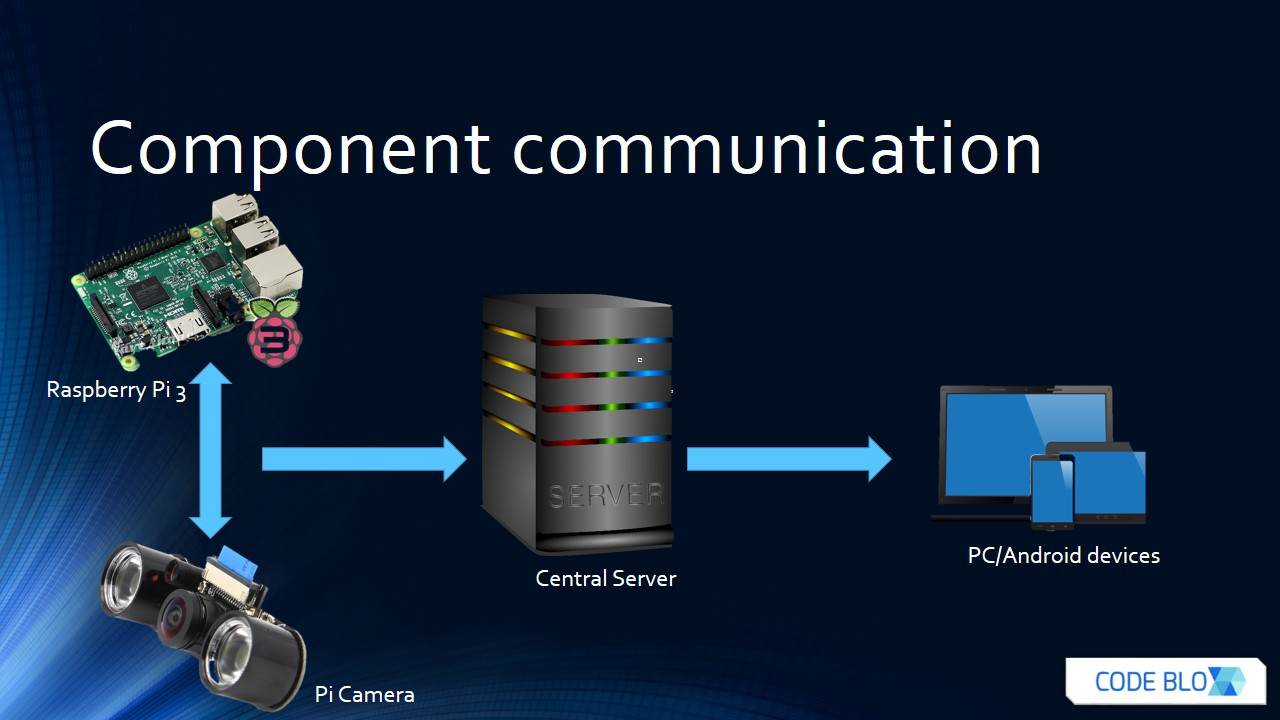
\includegraphics[width=1\textwidth]{./Pictures/CodeBlox.jpg}\\[1.5cm] 
	
		\subsection{Raspberry Pi 3}
		The Raspberry Pi is used to serve the purpose of the client. It handles all the requests passed down from the main server which include open/close gate, getting camera feed and handling other appliances in the system.
		
		\subsection{Pi Camera}
		The camera is simply used to stream a live video from the house to the owner.
		
		\subsection{Central Server}
		The central server is used to connect the user to their house from any location in the world as long as a live internet connection exists.
		
		\subsection{PC/Android devices}
		The live video is streamed to these devices and is also used as a remote to control the devices in the house.
		
	\section{Installation}
	
		\subsection{Software}
			\subsubsection{NodeJs}
			Install by using the following command: \newline
			\textbf{sudo apt-get install nodejs}
			\subsubsection{NPM(Node package manager)}
			We have used npm to install our node packages. It can be installed using: \newline
			\textbf{sudo apt-get install npm}
			\subsubsection{Installing dependencies}
			When working with nodejs, a package.json file is created whereby all the application dependencies are listed. The list for the dependencies can be found on our git repo at:
			\textbf{https://github.com/billibongers/CodeBlox---Main-Project/blob/master/Code/NodeJs\newline/personModule/package.json}
			\newline\newline
			To automatically install all dependencies run the command:\newline
			\textbf{npm install}
			
			\subsubsection{Connecting to private network}
			Download OpenVpn form google play store at:\newline \textbf{https://play.google.com/store/apps/details?id=net.openvpn.openvpn\&hl=en} \newline\newline
			Install Openvpn and browse to the homeautomation.codeblox.co.za ca certificated that was provided to you by CodeBlox \newline
			Connect to the Vpn via the connect buttom then open the Dropoff app. \newline\newline
			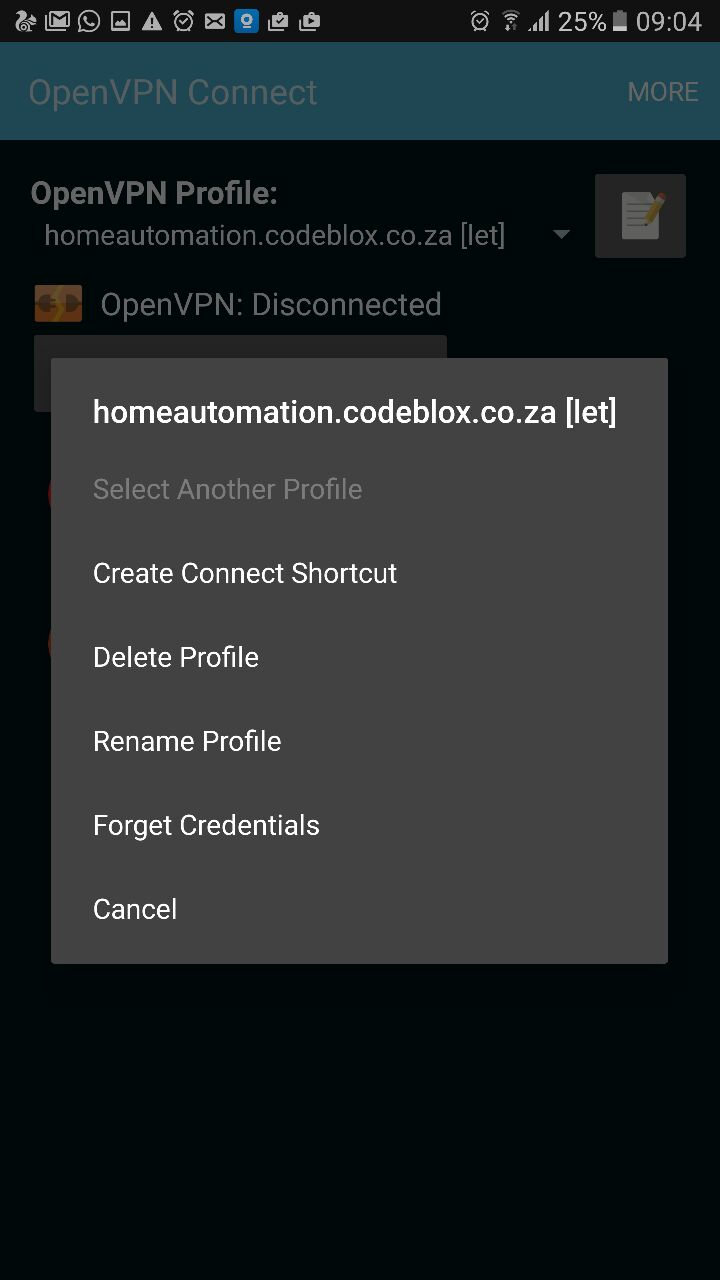
\includegraphics[width=10cm,height=10cm,keepaspectratio]{./Pictures/open2.jpeg}
			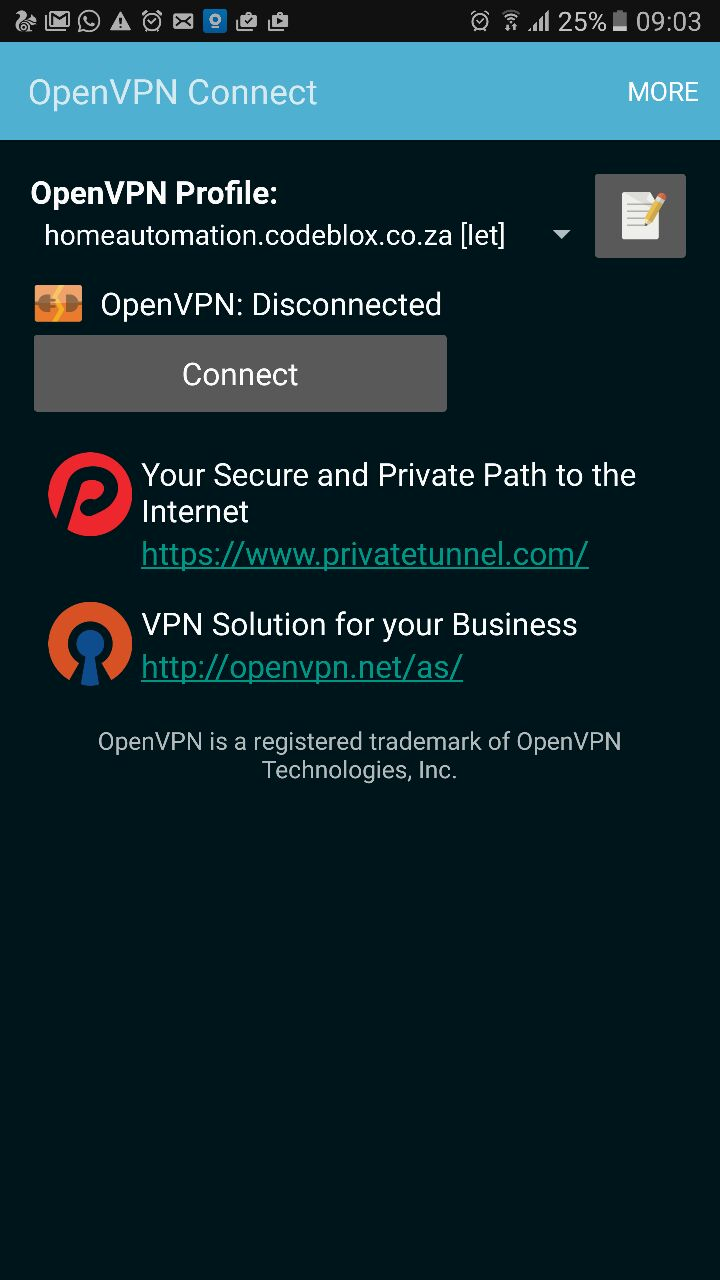
\includegraphics[width=10cm,height=10cm,keepaspectratio]{./Pictures/open1.jpeg}\\ 
			
			
			\subsubsection{Installing application on andorid device}
			The android application is coded in Android Studio using pure java. It can be found in our Android git repo which is dedicated to the mobile app here:
			\textbf{https://github.com/lspazzoli\newline/CodeBlox-Android}
			\newline\newline
			The following is a graphical representation of how to install the application on a mobile phone once downloaded from the abovementioned URL
			
			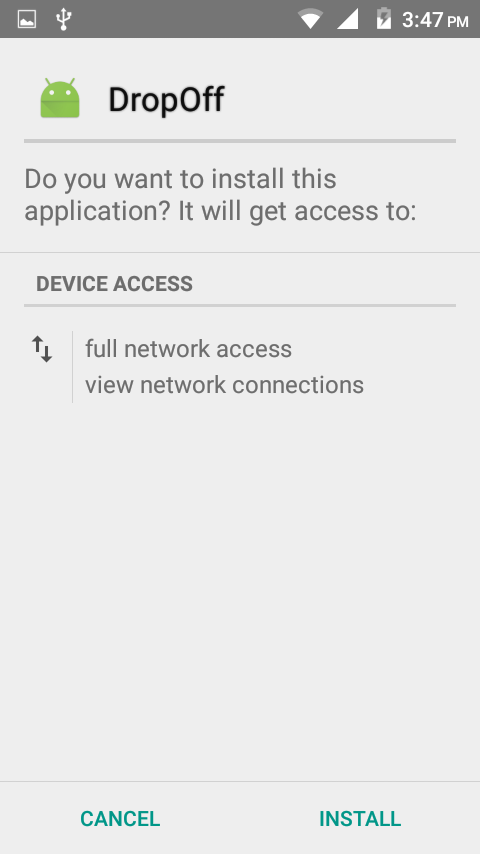
\includegraphics[width=10cm,height=10cm,keepaspectratio]{./Pictures/install1.png}
			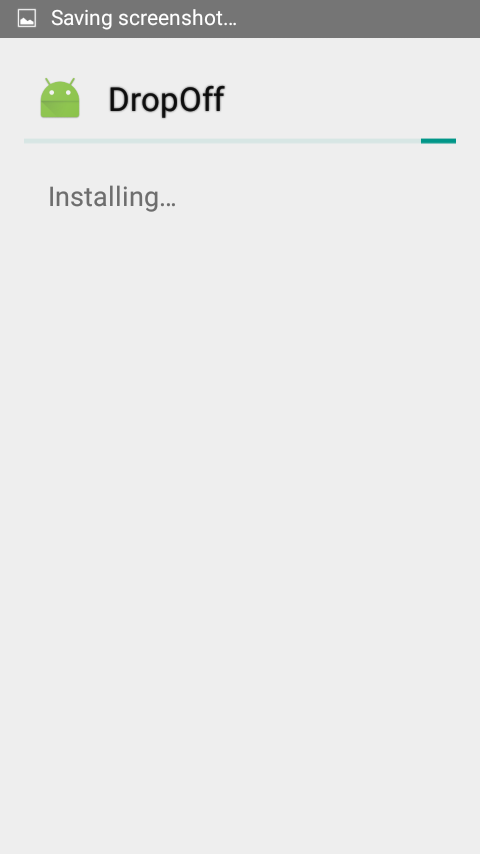
\includegraphics[width=10cm,height=10cm,keepaspectratio]{./Pictures/install2.png}
			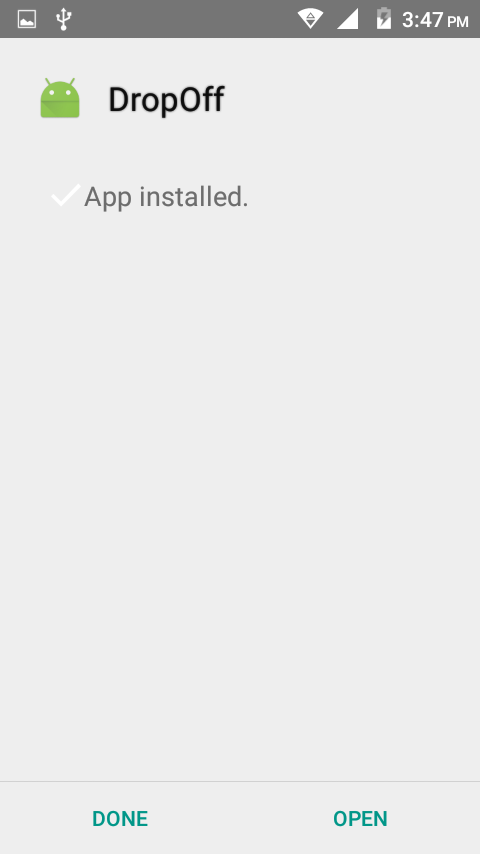
\includegraphics[width=10cm,height=10cm,keepaspectratio]{./Pictures/install3.png}\\
			Once the .apk has been clicked on, Step 1 appears telling you the permissions, these permissions are required to communicate with the pi and camera, they are networking permissions only. Step 2 installs the program and step 3 confirms the installation was successful\newline\newline
			
			\subsubsection{Application Information}
			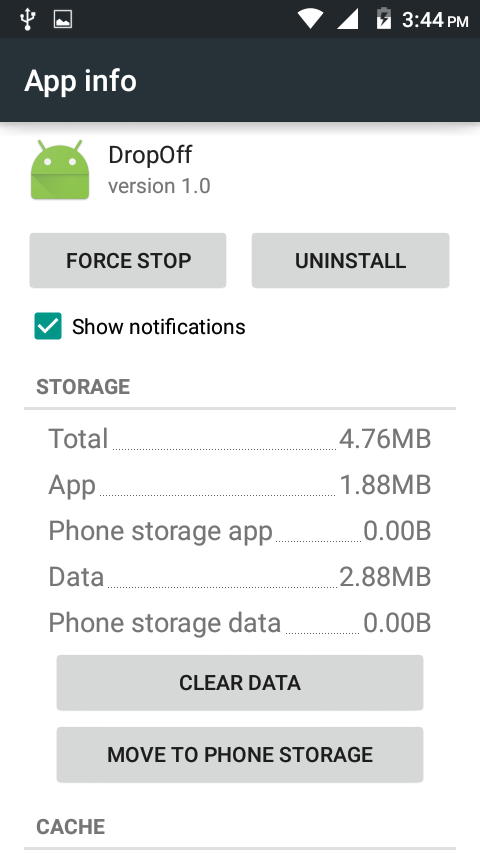
\includegraphics[width=10cm,height=10cm,keepaspectratio]{./Pictures/appinfo.png}\\
			The app is light weight, it uses less than 10mb of internal storage, this is so that it may run on low cost devices. The current version is 1.0 this is because the application has just entered its beta stages for the demo 2. The version 0.x was used for alpha and 2.x will be used for the actual release
				
		\subsection{Hardware}
		A CodeBlox technician will be sent out to install the hardware at your residence 
	\section{Getting Started}
		\subsection{Creating Account}
		Browse to \textbf{http://homeautomation.codeblox.co.za/} and click on register. \newline\newline 
		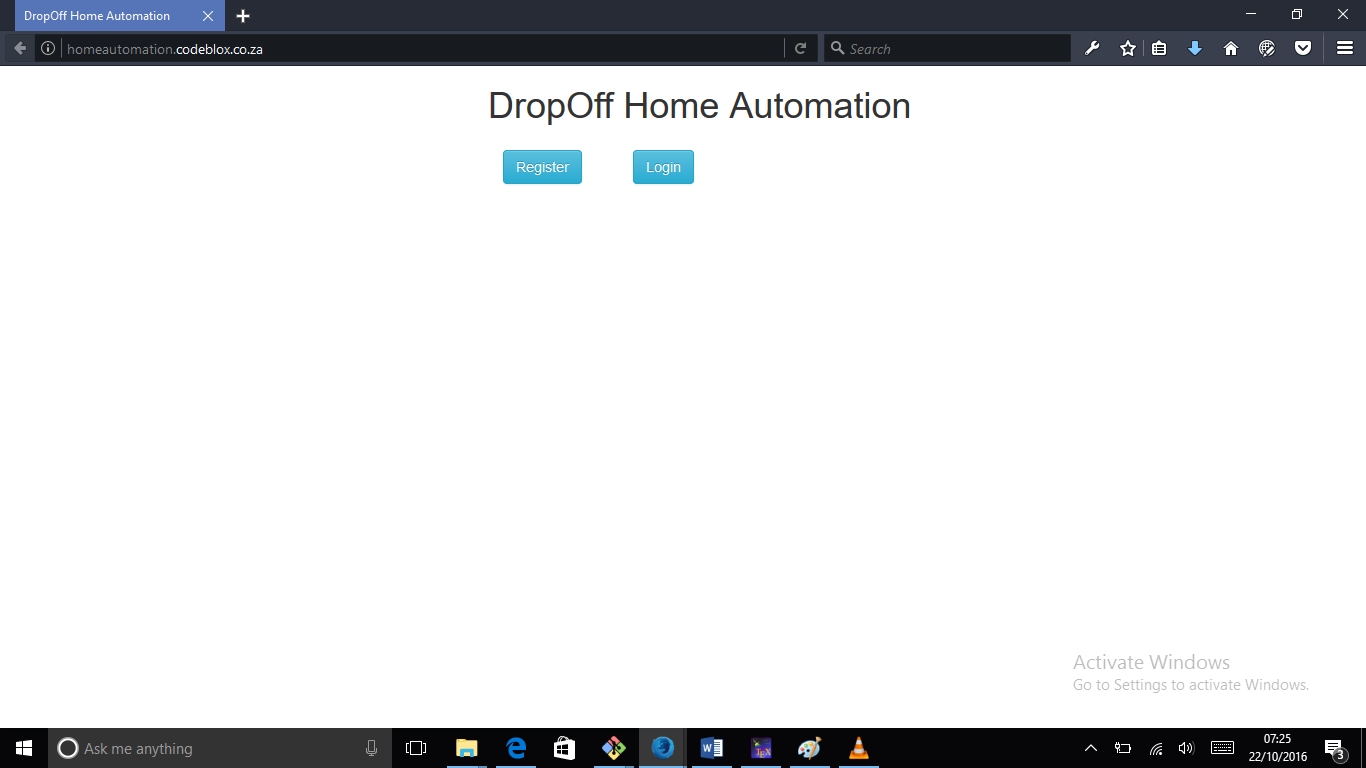
\includegraphics[width=10cm,height=10cm,keepaspectratio]{./Pictures/register.png}\newline
		After registration the CodeBlox team will contact you to arrange installation day.\newline\newline
		If you have an active account you may login and access all the functionality from the browser.
			
	 \section{Using the system}
	 Open application by touching the icon \newline\newline
	 	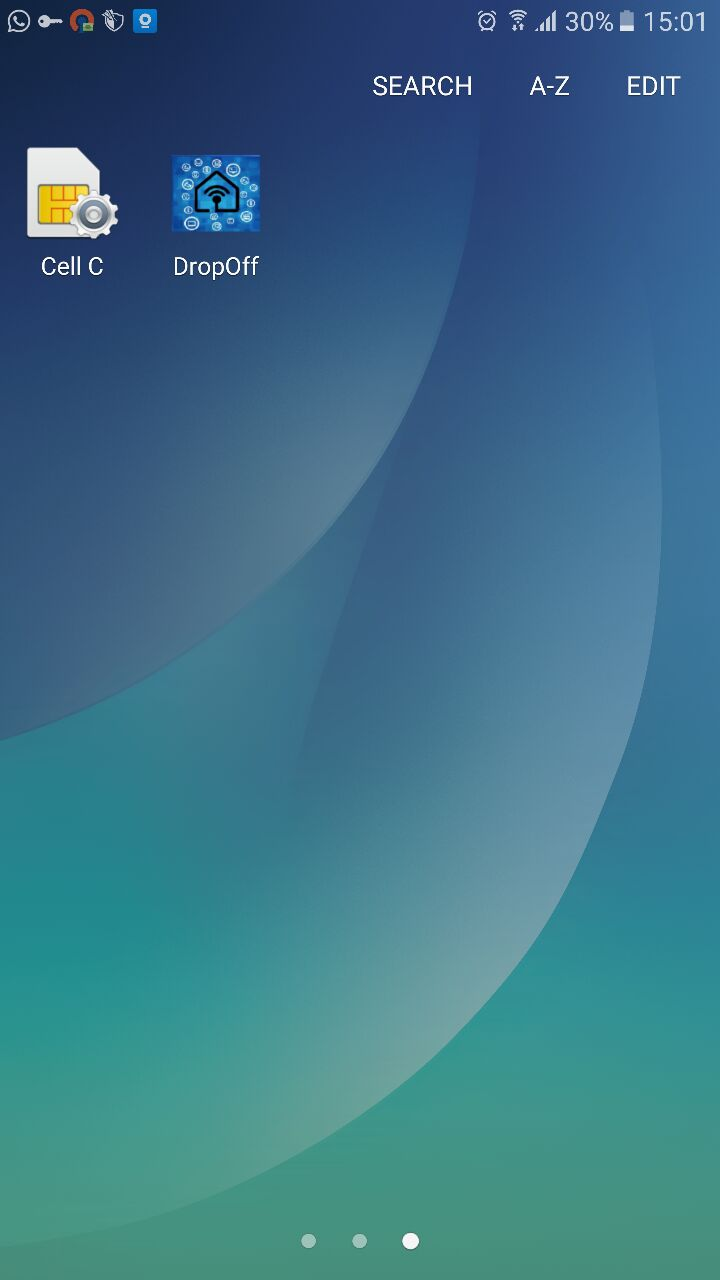
\includegraphics[width=10cm,height=10cm,keepaspectratio]{./Pictures/app0.jpeg}\\ \newline
	 The app will display a splash page while it is loading. The application will then prompt you to enter the server ip address and video stream url\newline\newline
	 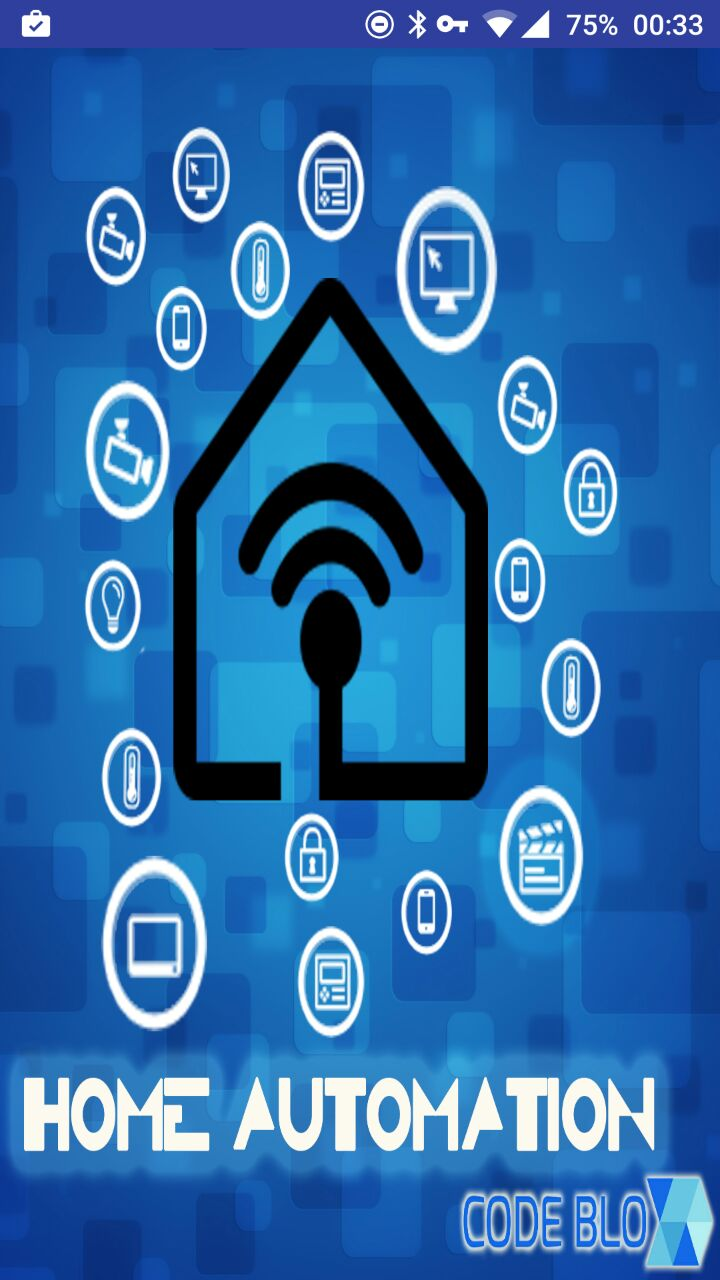
\includegraphics[width=10cm,height=10cm,keepaspectratio]{./Pictures/app01.jpeg}
	 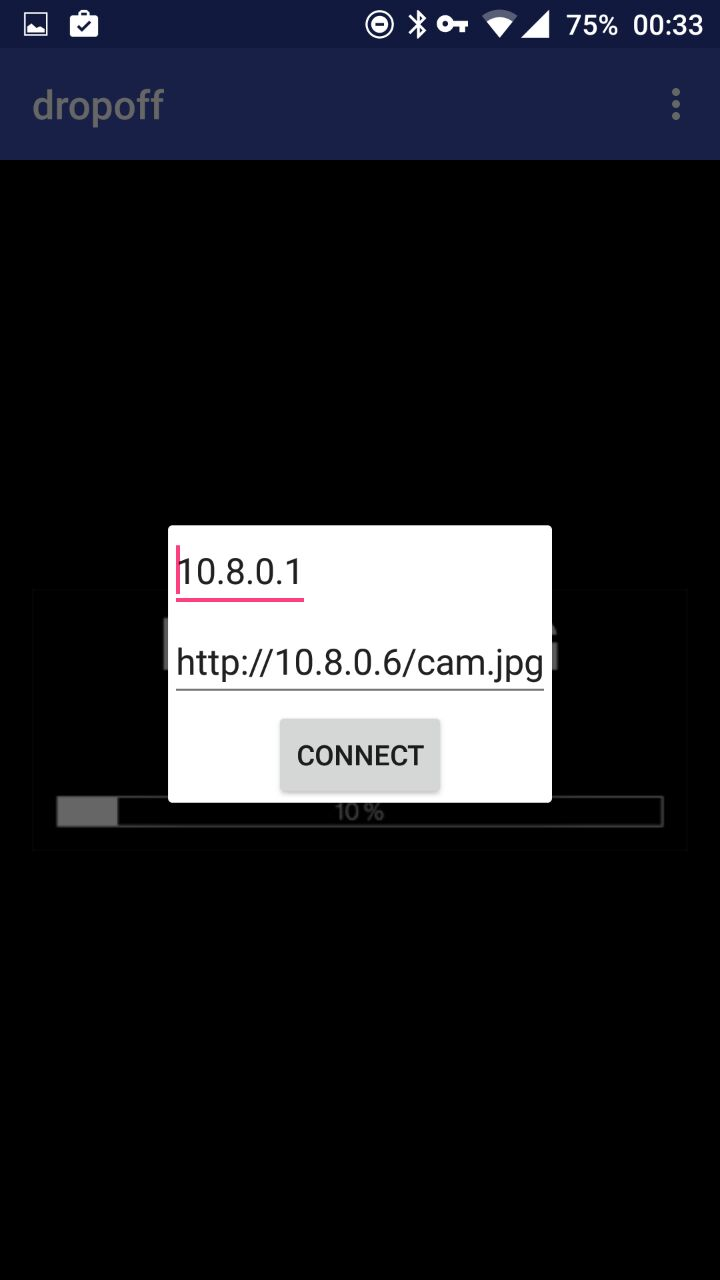
\includegraphics[width=10cm,height=10cm,keepaspectratio]{./Pictures/app1.jpeg}\\ \newline
	 After entering the details the application will load the video stream. Press the drop down menu to view all options that you have. Select the option of your choice and view effect on the live stream\newline\newline 
	 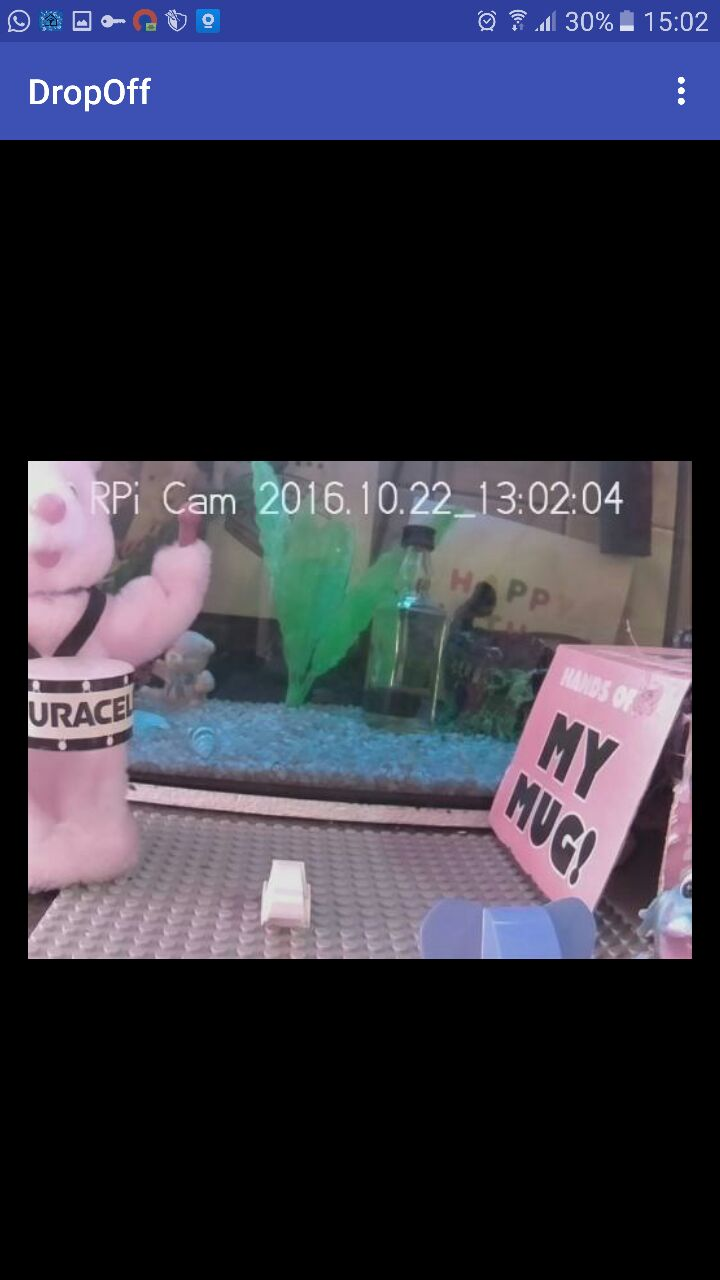
\includegraphics[width=10cm,height=10cm,keepaspectratio]{./Pictures/app2.jpeg} 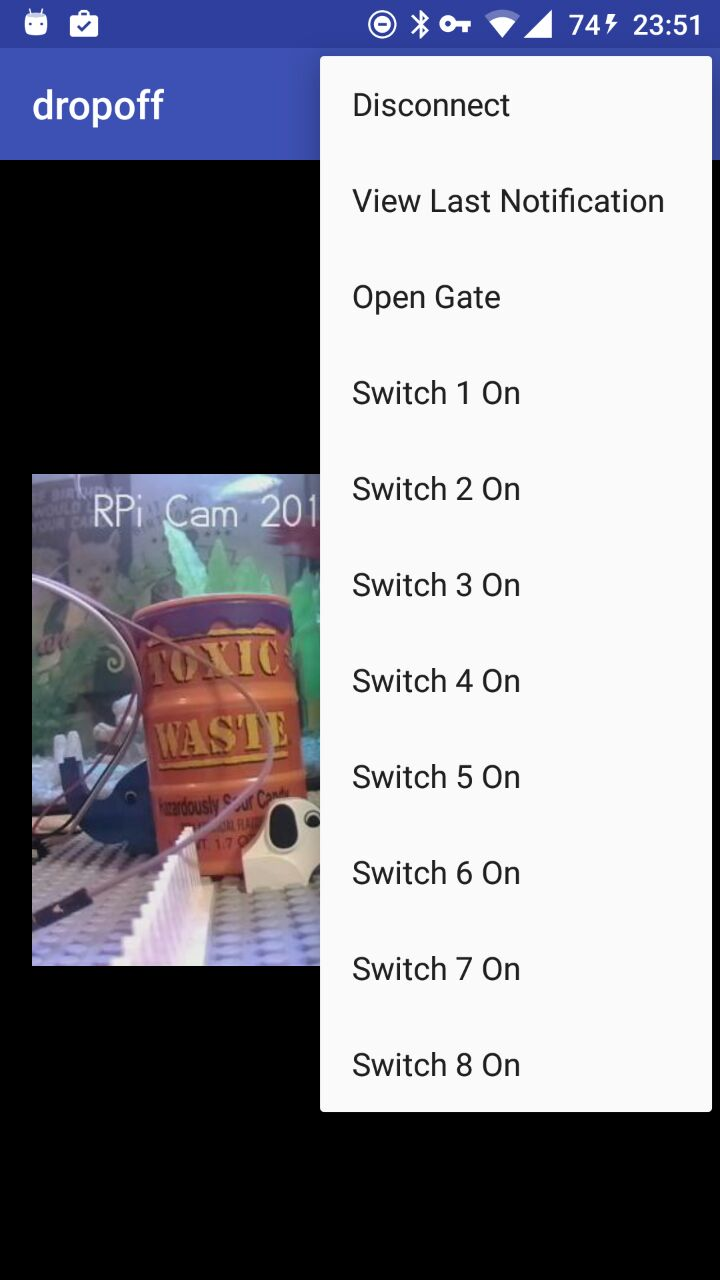
\includegraphics[width=10cm,height=10cm,keepaspectratio]{./Pictures/app3.jpeg}\\
	 
	 \subsection{Disconnect}
	 This button will disconnect you from the server, meaning you will not be able to control anything in your house. However, the video will still stream live.
	 \subsection{View Last Notification}
	 This button will display a pop up with a notification from the server.
	 \subsection{Open gate / Close gate}
	 This button will open/close the gate based on the status.
	\subsection{Switch 1 On}
	This button will turn the plug on, turning on the appliance at that specific switch.\newline\newline
	These buttons are client specific,hence they many range in number.
	
	\section{Troubleshooting}
	The down-time of our server around 10 seconds and it takes about 30 seconds for the home pi to reconnect. Hence if our main system crashes, it will take you less then a minute to reconnect. Given that you are using the application, otherwise it will reconnect automatically.

\end{document}